\chapter{Εισαγωγή}

Με την αυγή της τρίτης δεκαετίας του εικοστού πρώτου αιώνα, έχει καταστεί
σαφές πως οι υπηρεσίες του \en{cloud computing} αποτελούν ένα από τα
ισχυρότερα εργαλεία της σύγχρονης τεχνολογίας των υπολογιστών. Ως εκ τούτου,
αποτελεί αντικείμενο σχολαστικής μελέτης από πανεπιστημιακά ιδρύματα και
ερευνητικά κέντρα παγκοσμίως.
Ο όρος \en{cloud computing} αναφέρεται σε ένα αφηρημένο μοντέλο υπολογιστικών δομών ανεξάρτητό
από τα φύσικό υλικό (\en{hardware}) όπου γίνονται οι υπολογισμοί, σε αντίθεση με τα παραδοσιακά
\en{IT infrastructure} όπου το υλικό είναι άμεσα προσβάσιμο και αλληλένδετο με την εκάστοτε
επεξεργαστική δραστηριότητα.
Το μεγάλο πλεονέκτημα του \en{cloud computing},
είναι η \en{on-demand} πρόσβαση σε υπηρεσίες ή και υπολογιστικούς
πόρους χωρίς την άμεση εμπλοκή της χρήστη, από απομακρυσμένο περιβάλλον\cite{wikipediaCloud}.
\newline

Το \en{cloud computing} στηρίζεται σε μεγάλο βαθμό στην εικονικοποίηση (\en{virtualization}).
Με τον όρο εικονικοποίηση περιγράφεται η διαδικασία εκτέλεσης ενός εικονικού
(σε αντιδιαστολή με το πραγματικό) στιγμιοτύπου ενός υπολογιστικού συστήματος, σε
αφαίρεση από το πραγματικό υλικό επάνω στο οποίο γίνεται η εκτέλεση.
Υπάρχουν διάφορα είδη εικονικοποίησης. Ένα αρκετά γνωστό στον μέσο προγραμματιστή
είδος είναι η εικονικοποίηση σε επίπεδο εφαρμογών, όταν η γλώσσα
προγραμματισμού επιβάλει την εκτέλεση της εφαρμογής εντός εικονικού περιβάλλοντος,
π.χ. η \en{java} με το \en{JVM}\cite{JVM}. Ένα στιγμιότυπο εικονικοποίησης και προσομοίωσης
ενός υπολογιστικού συστήματος ονομάζεται εικονική μηχανή (\en{virtual machine} ή \en{VM}).
Η παρούσα διπλωματική εργασία ασχολείται με την εικονικοποίηση σε επίπεδο
συστήματος, όπου το σύνολο του υλικού του συστήματος εικονικοποιείται με την
βοήθεια κάποιου επόπτη (\en{hypervisor}). Τέτοιοι επόπτες είναι συνήθως το \en{KVM},
το \en{Xen} κ.α.
\newline
\begin{figure}[h]
  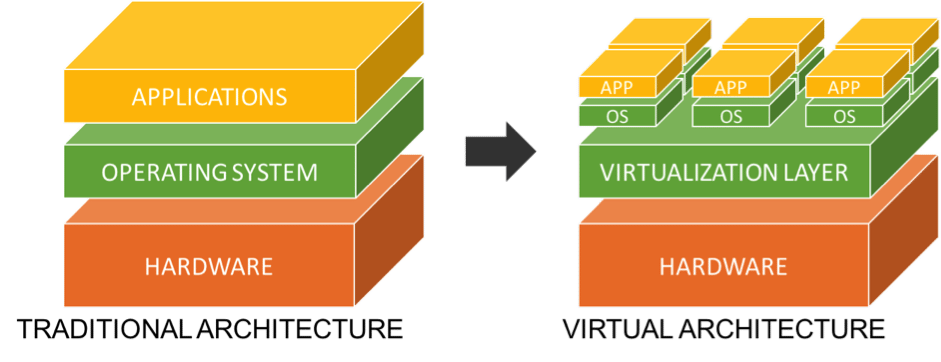
\includegraphics[width=0.7\textwidth]{pictures/generalVirtulization.png}
  \caption{Παραδοσιακό σύστημα και Εικονοποιημένο σύστημα}
  \label{fig:generalVirtulization}
\end{figure}

Ο επόπτης είναι ένα σύνολο λογισμικού, το οποίο επιτρέπει την
εικονικοποίηση ενός συστήματος. Οι εποπτές μπορεί να είναι διεργασίες-μέρη ενός άλλου λειτουργικού συστήματος (\en{host})
ή να παρεμβάλλονται απευθείας ανάμεσα στο υλικό και το εικονοποιημένο σύστημα
(\en{guest}). Στην πρώτη περίπτωση ονομάζονται επόπτες τύπου II, ενώ στην δεύτερη
επόπτες τύπου I\cite{Aimilios}.
\newline
\begin{figure}[h]
  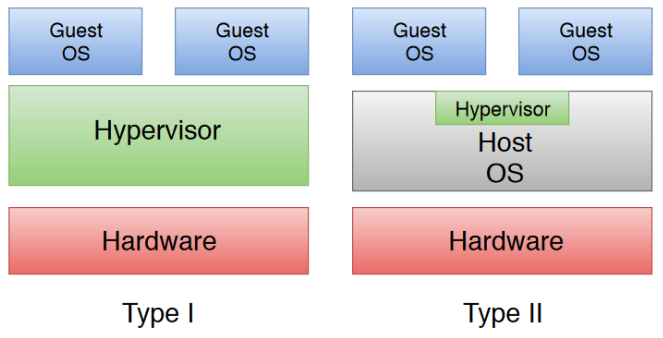
\includegraphics[width=0.7\textwidth]{pictures/typeI-II-hypervisors.PNG}
  \caption{Επόπτες τύπου I και τύπου ΙΙ}
  \label{fig:typeI-II}
\end{figure}


Ταυτόχρονα με την εικονικοποίηση, χρησιμοποιείται και τεχνική της προσομοίωσης
(\en{emulation}). Με την προσομοίωση, μπορεί να αναπαραχθεί πιστά η συμπεριφορά ενός
κομματιού υλικού, το οποίο δεν έχει κάποιο φυσικό αντίστοιχο στο υφιστάμενο πραγματικό
σύστημα. Τέτοια κομμάτια υλικού μπορεί να είναι, για παράδειγμα, μια κάρτα δικτύου. Η
αναπαραγωγή της συμπεριφοράς γίνεται εξ ολοκλήρου σε επίπεδο λογισμικού
(\en{software}). Ένα ευρέως διαδεδομένο πρόγραμμα προσομοίωσης είναι
το \en{QEMU (Quick EMUlator)},
το οποίο μπορεί να λειτουργήσει και ως επόπτης, ενώ ο συνδυασμός \en{emulator-hypervisor}
\en{QEMU/KVM} είναι
μια από τις αποτελεσματικότερες λύσεις για εικονικοποίηση της εκτέλεσης ενός
λειτουργικού συστήματος\cite{QemuWiki}.

\section{Είδη εικονικοποίησης}

Με την πλήρη εικονικοποίηση, προσομοιώνεται η λειτουργία ενός πλήρους λειτουργικού
συστήματος. Μια σημαντική ιδιότητα είναι πως δεν υπάρχει υποβοήθηση από το
υλικό \en{(hardware assisted)}, όπως εμφανίζεται σε άλλη περίπτωση στην συνέχεια.
Το λειτουργικό σύστημα που προσομοιώνεται (\en{guest}) δεν χρειάζεται να υποστεί
καμία αλλαγή και προσφέρεται ως έχει. Ο \en{hypervisor} προσφέρει οτιδήποτε
χρειάζεται ο \en{guest} σε επίπεδο υλικού, έτσι ώστε ο \en{guest} να αισθάνεται πως
εκτελείται επάνω σε πραγματικό υλικό, όπως είναι σχεδιασμένος να κάνει.
Ταυτόχρονα, προσομοιώνει και την εκτέλεση των εντολών του επεξεργαστή.
Ειδική μνεία χρειάζεται για τις προνομιούχες εντολές του \en{guest}, οι οποίες
δεν επιτρέπεται για λόγους ασφάλειας να εκτελεστούν απευθείας επάνω στην
\en{CPU}, και για αυτό τον λόγο εφαρμόζονται διαφορετικές λύσεις όπως η \en{trap and
emulate}. Μάλιστα, ειδικά για την \en{x86} αρχιτεκτονική, η δυσκολία στο να
προσομοιωθούν αυτές οι συγκεκριμένες εντολές έκαναν αρχικά την εικονικοποίηση να μοιάζει
αδύνατη \cite{VMwarePaper}.
\newline

H προηγούμενη τεχνική έχει το μειονέκτημα της μειωμένης ταχύτητας εκτέλεσης.
Για τον λόγο αυτό έχει αναπτυχθεί η εικονικοποίηση με υποβοήθηση υλικού
(\en{hardware assisted virtualization}), όπου έχουν προστεθεί εντολές στην \en{CPU},
οι οποίες βοηθούν την εκτέλεση του συνόλου των εντολών του \en{guest}, δίχως
μείωση  στην ταχύτητα. Και σε αυτήν την περίπτωση ο \en{guest} εκτελείται ως
έχει, χωρίς κάποια τροποποίηση, όμως υπάρχει πρόβλεψη από το υλικό ώστε να
επιταχύνει την εκτελεσή του με ασφάλεια\cite{VMwarePaper}. Αυτή η τεχνική είναι διαθέσιμη
εφόσον υπάρχουν επεκτάσεις υλικού (\en{virtualization extensions}), όπως η
τεχνολογία \en{VT-x} της \en{Intel} και \en{AMD-V} της \en{AMD} στους επεξεργαστές της εκάστοτε εταιρείας\cite{wikipediaX86}.
\newline

Επιπροσθέτως, η άγνοια του \en{guest}, ως προς την εκτέλεση του επάνω σε εικονικό
σύστημα, μπορεί μεν είναι μια πολύ επιθυμητή αφαίρεση, οδηγεί όμως συχνά σε
μη βέλτιστη συμπεριφορά και χρήση των πόρων του πραγματικού συστήματος. Για
παράδειγμα η διαχείριση της υφιστάμενης μνήμης \en{RAM}, δεν γίνεται με βέλτιστο
τρόπο, από μεριάς \en{guest}, καθώς δεν γνωρίζει πραγματικά πόση συνολικά διαθέσιμη
υπάρχει στο σύστημα, παρά μόνο τόση όση έχει ανατεθεί από τον \en{host} στον
\en{guest}.  Με την παρα-εικονικοποίηση (\en{paravirtualization}), ο \en{guest} γνωρίζει
πως δεν εκτελείται επάνω σε φυσικό σύστημα, και ζητά την συνεργασία του
επόπτη του για την αποδοτικότερη αντιμετώπιση συγκεκριμένων σεναρίων χρήσης
του. Επί παραδείγματι, o \en{guest} μπορεί να μεταβάλει την συμπεριφορά του και
να επιλέξει να μην εκτελέσει τις προαναφερθείσες ευαίσθητες εντολές, και
στην θέση τους να ζητήσει την συνεργασία του \en{host}, ώστε να αναλάβει αυτός
τις συγκεκριμένες εργασίες\cite{VMwarePaper}.

\section{Προβλήματα και λύσεις}

\subsection{\en{Unikernels}}

Οι περισσότερες υπηρεσίες στο \en{cloud computing} μπορούν εύκολα να υλοποιηθούν
ως απλές εφαρμογές ενός παραδοσιακού λειτουργικού συστήματος. Το \en{workload}
αυτών, είναι χαμηλών η μέτριων απαιτήσεων εστιασμένες στην εκάστοτε απαίτηση
του χρήστη-πελάτη. Όμως η δημιουργία μια εικονικής μηχανής στην οποία να
εκτελείται ένα συμβατικό λειτουργικό σύστημα είναι κάθε άλλο παρά τέλεια
λύση. Τα λειτουργικά είναι σχεδιασμένα με γνώμονα την παράλληλη εκτέλεση
πολλαπλών εφαρμογών, είναι υπερβολικά σύνθετα, και πολύ αργά στην εκκίνηση
για τις απαιτήσεις των στιγμιαίων υπηρεσιών του \en{cloud}. Το κυριότερο
όμως, είναι πως η πολυπλοκότητα του συστήματος είναι αχίλλειος πτέρνα
για την ασφάλεια και την σταθερότητα ολόκληρης της εικονικής μηχανής.
\newline

Λύση στο ανώτερο πρόβλημα προσφέρουν τα \en{unikernels}, μικρές εικονικές μηχανές
ικανές να εξουδετερώσουν τις προαναφερθείσες αδυναμίες. Εστιασμένα στην εκτέλεση μιας
συγκεκριμένης υπηρεσίας έχουν ελάχιστες απαιτήσεις σε υλικό, ενώ
διατηρούν τάξεις μεγέθους μικρότερο μέγεθος από τα παραδοσιακά λειτουργικά.
Επιπροσθέτως, η μείωση της πολυπλοκότητας τους και του μεγέθους αυτών,
μειώνει την πιθανότητα δυσλειτουργίας καθώς και την επιφάνεια επίθεσης
(\en{attack surface}) από κακόβουλους τρίτους χρήστες\cite{unikernelsDef}. Υπάρχουν διάφορα
\en{unikernel frameworks}, τα οποία θα αναφερθούν αργότερα, ενώ οι εικονικές
μηχανές που προέρχονται από αυτά συνήθως εκτελούνται με την βοήθεια
κάποιου επόπτη ή πιο σπάνια απευθείας επάνω στο υλικό (\en{bare metal}).

\subsection{\en{Transcedent memory}}

Ένα δεύτερο πρόβλημα που αναφέρθηκε είναι η υποχρησιμοποίηση των πόρων
του συστήματος στην περίπτωση του \en{virtualization}, και ειδικά της
μνήμης. Όταν εξαντληθεί η διαθέσιμη μνήμη, ένα παραδοσιακό λειτουργικό
καταφεύγει στο να μεταφέρει (\en{swapping}) σελίδες μνήμης (\en{memory pages}),
στον δίσκο ή σε κάποιο αντίστοιχο αποθηκευτικό μέσο, η ταχύτητα των
οποίων είναι πολύ μικρότερο σε σχέση με της φυσικής μνήμης. Κατά
την εικονικοποίηση ενός \en{VM} το πιθανότερο όμως είναι να υπάρχει
διαθέσιμη φυσική μνήμη, απλά όμως να ανήκει στον \en{host}, και να μην
έχει ανατεθεί εξ αρχής στον \en{guest}. Άρα ένος μέρος της φυσικής μνήμης παραμένει
ανεκμετάλευτο, γεγονός που θα μπορούσε να έχει αποφευχθεί εάν η μνήμη κατανέμονταν
με αποδοτικότερους τρόπους.
\newline

Για να αντιμετωπιστεί αυτό το φαινόμενο έχουν εφαρμοστεί διάφορες
λύσεις, κάθε μια με διαφορετικά πλεονεκτήματα και μειονεκτήματα.
Μια ισορροπημένη τεχνική στηρίζεται στην εκμετάλλευση της  επικοινωνίας
\en{host} και \en{guest}, δηλαδή εφαρμογή τεχνικών \en{paravirtualization},
ώστε να μεταβάλλεται δυναμική η διαθέσιμη μνήμη του \en{guest}. Για
παράδειγμα, ο μηχανισμός του \en{ballooning} αυξομειώνει κατά το \en{runtime} τον αριθμό
σελίδων μνήμης που ανήκουν στον \en{guest}, σύμφωνα με τις ανάγκες του.
\newline

Η μηχανισμός πτητικής μνήμης (\en{transcendent memory} ή \en{tmem}), ο οποίος
αναπτύχθηκε από την \en{Oracle} το 2009, επεκτείνει την τελευταία σκέψη
συνεργασίας \en{guest-host} ένα βήμα παραπέρα. Ο \en{guest} σε περίπτωση έλλειψης
μνήμης δεν ζητά να του παραχωρηθεί επιπλέον από τον \en{host}, αλλά ζητά
από ο \en{host} να αναλάβει αυτός την αποθήκευση των δεδομένων του που
έχει στην μνήμη, ωστέ στη συνέχεια αυτός να μπορεί να αποδεσμεύσει μέρος
της μνήμης του γνωρίζοντας πως ανά πάσα στιγμή μπορεί να την ανακτήσει
από τον \en{host}  Η αναφορά σε αυτές τις περιοχές μνήμης γίνεται με ζεύγη
κλειδιού-τιμής (\en{key-value}), ώστε \en{host} και \en{guest} να έχουν ένα κοινό
κώδικα-πρωτόκολλο επικοινωνίας\cite{tmemXenSummit}\cite{Aimilios}.
\newline

Στην \en{tmem}, η επικοινωνίας γίνεται μεταξύ του πυρήνα (\en{kernel space})
του \en{host} και του \en{guest}. Σε προηγούμενη διπλωματική, όμως, ο μηχανισμός
έγινε άμεσα προσβάσιμος από το χώρο χρήστη (\en{user space)} του \en{guest}, και άρα
από τις εκτελούμενες εφαρμογές, και ονομάστηκε \en{userspace transcendent
memory} ή \en{utmem}. Αποδείχθηκε δε, πως σε περιπτώσεις έλλειψης μνήμης μια
εφαρμογή που χρησιμοποιεί αυτόν τον μηχανισμό παρουσιάζει καλύτερη
συμπεριφορά ως προς την ταχύτητα και την διαχείριση της μνήμης\cite{paperAimiliou}.

\section{Σκοπός της εργασίας}

Ο σκοπός αυτής της διπλωματικής είναι η μελέτη των \en{unikernel frameworks}
και του μηχανισμού \en{utmem}. Στην συνέχεια παρουσιάζουμε την ενσωμάτωση του
μηχανισμού της \en{utmem} σε ένα συγκεκριμένο \en{unikernel framework}, καθώς και
την πειραματική αποτίμηση της νέας διαθέσιμης τεχνολογίας σε σύγκριση με
τα υπάρχοντα δεδομένα.
\newline

Με την παρούσα εργασία, αναπτύσσουμε ένα αξιόλογο εργαλείο για τον
προγραμματιστή \en{unikernel} εφαρμογών, όσον αφορά την ρητή διαχείριση
της μνήμης των εφαρμογών του. Ταυτόχρονα, όπως φαίνεται και στην συνέχεια,
βελτιώνουμε την συμπεριφορά του \en{unikernel} σε σενάρια έλλειψης διαθέσιμης μνήμης.
